\section{OpenVPN}
\subsection{Overview}
OpenVPN è un software open source molto diffuso per la creazione di VPN,
è in grado di incapsulare pacchetti al livello 2 o 3, e come protocollo di trasporto
può usare TCP o UDP. E' la soluzione che è stata scelta, ed in questo capitolo
se ne presenta una panoramica, mentre viene approfondita nel dettaglio
nel prossimo.


Per ciascun tunnel VPN, vengono create due connessioni separate:
\begin{itemize}
  \item \texttt{Control Channel} cifrato con TLS per scambiarsi informazioni di servizio
  \item \texttt{Data Channel} cifrato con un protocollo simile  a TLS per lo scambio
  di dati.
\end{itemize}
Entrambe le connessioni sono multiplexate su di un unico protocollo di trasporto
da OpenVPN, sia esso TCP o UDP.
OpenVPN è una tecnologia ampiamente usata per creare VPN.
La figura \ref{fig:openvpn-sec} mostra un semplice schema del suo funzionamento.\\
\begin{figure}[h!]
  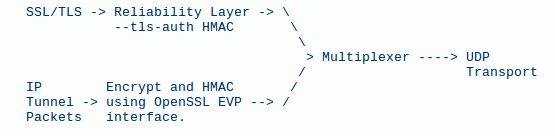
\includegraphics[scale=0.4]{img/openvpn_sec}
  \caption[Il multiplexing di OpenVPN]{Il multiplexing di OpenVPN: si vede come
  le due connessioni siano multiplexate su un unico protocollo L4, in questo caso UDP.}
  \label{fig:openvpn-sec}
\end{figure}
OpenVPN viene distribuitpo anche in una versione \textit{enterprise} a pagamento: si chiama
\textit{OpenVPN AS -- Access Server}, offre una web GUI, sicuramente più intuitiva
rispetto ai file di configurazione con cui si amministra la versione open source
(detta \textit{Community Edition}). D'ora in poi ci si concentra su quest'ultima
versione, a livello di VPN le funzionalità sono le stesse; per una comparazione tra
le due versioni si veda
\cite{openvpn-comparison}.\\
L'infrastruttura OpenVPN si compone di:
\begin{itemize}
  \item server: in grado di connettere tra loro diversi client, è possibile regolare
  il fatto che diversi client possano \textit{vedersi} tra loro o meno
  \item client, il quale si connette al server.
\end{itemize}
E' necessario che il server abbia un indirizzo IP pubblico, oppure dinamico e raggiungibile con un DNS. E' possibile
usare servizi che dinamicamente seguono gli aggiornamenti agli indirizzi IP, in modo che i client usino
sempre un unico nome per raggiungerlo. Si noti che questa tecnologia (\textit{dynamic DNS}) è integrata in SoftEther.\\
E' possibile avere il server dietro un firewall, a patto di abilitare il port forwarding dal gateway al server.\\
L'autenticazione tra i diversi membri della VPN può essere fatta in due modi:
\begin{itemize}
  \item certificate-based, cioè autenticazione basata su chiavi pubbliche e certificati
  X509. I passi da seguire sono:
  \begin{itemize}
    \item creazione di una nuova CA, quindi della coppia di chiavi e di un certificato
    self-signed
    \item ciascun membro della VPN deve avere la propria coppia di chiavi e certificato
    \item il certificato della CA deve essere presente in ogni macchina partecipante
  \end{itemize}
  \item PSK: si generano a priori delle chiavi statiche, che devono essere distribuite
  su ciascun host membro della VPN. Questa modalità non è consigliata, in quanto
  se un host venisse in qualche modo compromesso, occorrerebbe cambiare tutte le chiavi.
  Inoltre non si garantisce \textit{perfect forward secrecy}: se un avversario
  intercettasse il traffico sull VPN e poi ottenesse queste chiavi potrebbe
  decifrarlo senza problemi.
\end{itemize}
E' possibile inoltre configurare anche username e password per ciascun client.

Si possono realizzare sia topologie \textit{Remote Access} sia \textit{LAN-to-LAN},
per ciò che concerne la configurazione effettiva di OpenVPN, le due cose
sono praticamente identiche, se si vuole realizzare l'ultima topologia occorre
però definire diverse rotte nelle reti partecipanti. In particolare,
l'host VPN (client o server) deve essere configurato come gateway per le reti
raggiungibili mediante l'\textit{altro} host VPN a cui è connesso.

Per ciò che concerne la versione free di OpenVPN, client e server sono implementati
nello stesso singolo programma.

\subsection{OpenVPN e MoonCloud}
Si passa ora ad analizzare le possibilità di implementare OpenVPN in MoonCloud al livello 3. Il primo step
da fare è decidere dove posizionare il server: nel cloud o nella rete target?
\begin{description}
  \item[\textbf{Nel cloud}]Con questa opzione si preparano nella rete MoonCloud una serie
  di VM destinate ad essere VPN server; se esse sono configurate propriamente, ciascun server
  può servire diverse reti target. I probes
  hanno delle rotte configurate del tipo \texttt{rete target via VPN server}.
  Nelle reti dei client si porta quindi una appliance che quindi client di un server in MoonCloud.
  Tale appliance deve rendere visibile l'intera rete (possibilmente anche più di una) nella VPN. In
  particolare si pone un problema di routing nella rete target a prescindere che lì vi sia
  il server od il client, pertanto è descritto tra qualche riga.
  \item[\textbf{Nella rete target}]Portare un server nella rete target subito un problema: deve
  essere raggiungibile dall'esterno, e questo non è per niente facile poiché la maggior parte
  delle reti target utilizzano NAT, e quindi gli host interni non sono direttamente raggiungibili
  dall'esterno, se non con port forwarding sul router. Chiedere ai clienti di configurare
  questo non è pensabile, pertanto questa opzione non è stata consigliata ed infatti
  non è stata presa effettivamente in considerazione come soluzione praticabile.
  In via del tutto ipotetica, se si fosse scelta questa strada si sarebbe poi
  dovuto decidere anche come effettivamente configurare i client VPN. Ad esempio,
  sarebbe stato possibile connettere direttamente al server ciascun Docker host, oppure
  dedicare un host al compito apposito di servire i vari Docker host nel collegamente VPN.
\end{description}
Il problema comune ad entrambe queste due opzioni è il seguente: in una configurazione
\textit{normale} i pacchetti provenienti dai probes e diretti ai target, una volta che
sono decifrati ed immessi nella rete dal VPN client (poiché l'opzione server
è stata scartata) hanno come indirizzo IP sorgente un IP che si trova nella rete MoonCloud,
ed i target non hanno modo di sapere che le risposte a tali pacchetti devono passare
per il VPN client. La soluzione a cui avevo già pensato in questa prima fase di studio
è stata quella del \textit{NAT al contrario}, per cui i pacchetti immessi nella rete
target dal VPN client vengono NAT-tati ed hanno come IP sorgente quello del VPN
client, che si trova nella stessa rete dei target e quindi le risposte torneranno
ad esso direttamente.

Senza NAT l'unica strada sarebbe stata configurare delle rotte sul default gateway
della rete target o su tutti gli host. In ogni caso, questa assieme a tutte
le altre soluzioni adottate per la VPN sono descritte molto dettagliatamente
nel prossimo capitolo.

% \begin{figure}
%   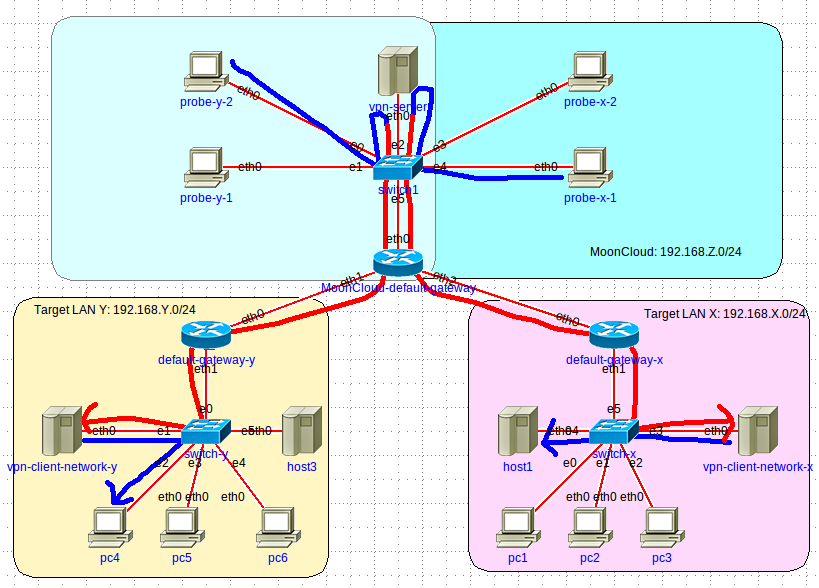
\includegraphics[scale=0.35]{img/sls}
%   \caption[Configurazione \textit{SLS (Single Local Server)}]{Configurazione \textit{SLS (Single Local Server)},
%   il server è in grado di collegare subnet con indirizzi IP diversi, a patto che tutto
%   sia configurato opportunamente. Le frecce rosse indicano il collegamento VPN, le frecce blu il traffico prima di essere inviato
%   e dopo essere stato decifrato dalla VPN.}
% \end{figure}

% \begin{figure}
%   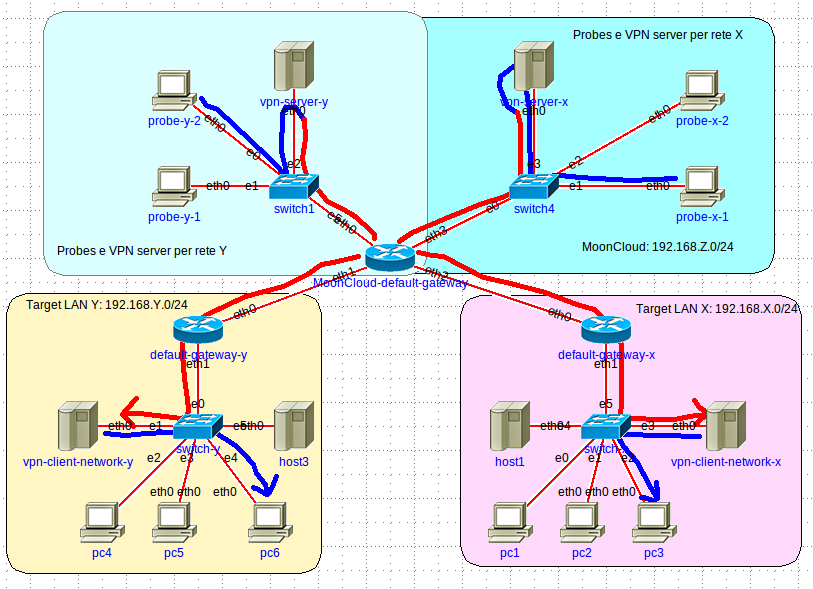
\includegraphics[scale=0.4]{img/mls}
%   \caption[Configurazione \textit{MLS (Multi Local Server)}]{Configurazione \textit{MLS (Multi Local Server)},
%   per ciascuna rete target si configura un VPN server che instrada il traffico dei containter (in blu) sulla VPN (in rosso).}
% \end{figure}

% \begin{figure}
% %   \centering
% %   \begin{minipage}[t]{0.5\textwidth}
%   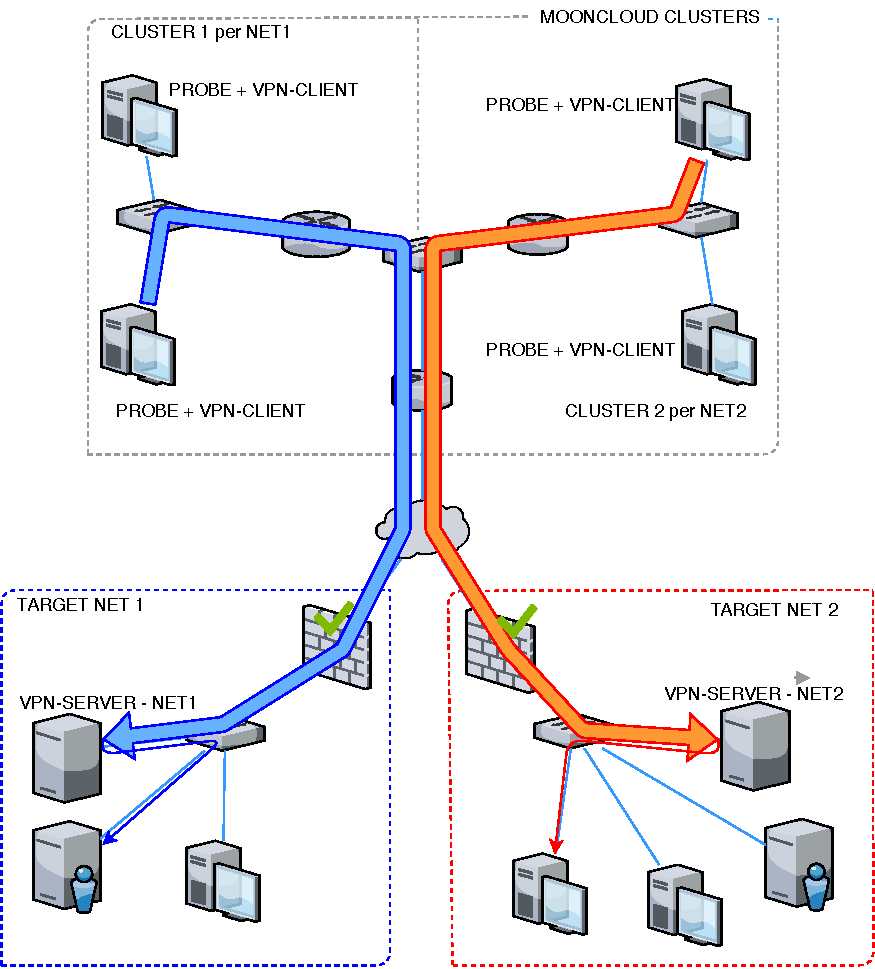
\includegraphics[scale=0.45]{img/rsmc}
%   \caption[Configurazione \textit{RSMC (Remote Server Multi Client)}]{Configurazione \textit{RSMC (Remote Server Multi Client)}.}
% \end{figure}
%   % \end{minipage}
%   % \hfill
%   % \begin{minipage}[t]{0.45\textwidth}
% \begin{figure}
%   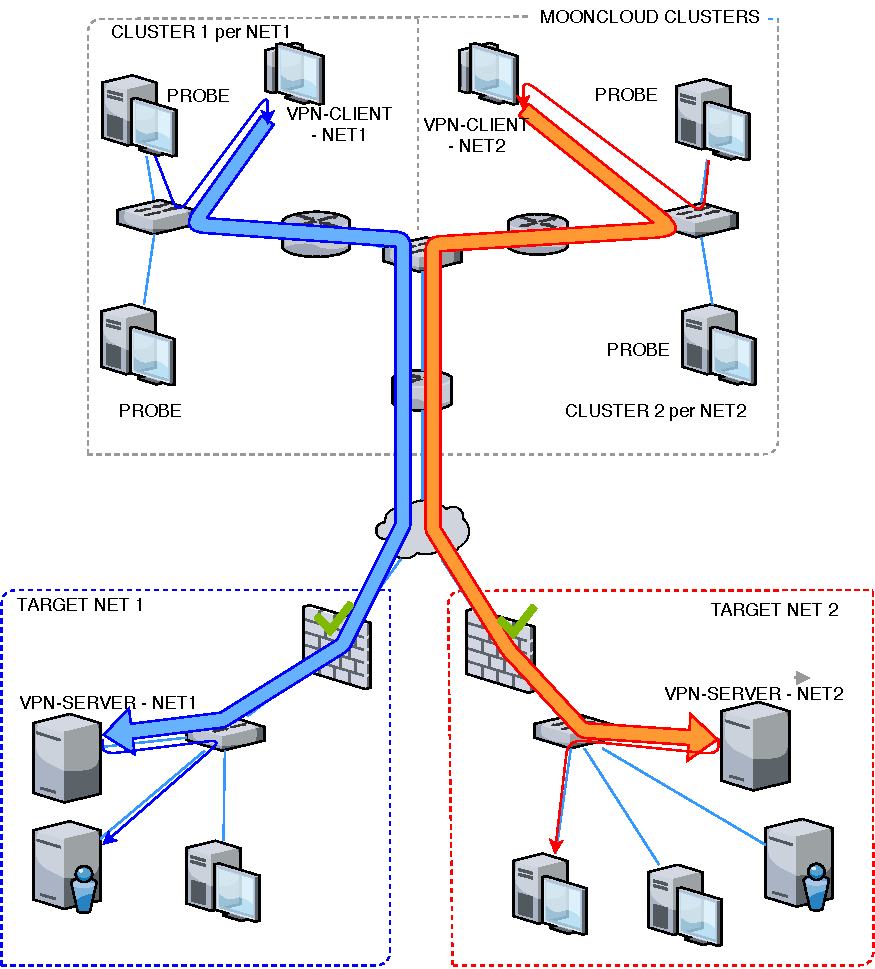
\includegraphics[scale=0.45]{img/rssc}
%   \caption[Configurazione \textit{RSSC (Remote Server Single Client)}]{Configurazione \textit{RSSC (Remote Server Single Client)}.}
%   % \end{minipage}
% \end{figure}

\subsection{Conclusioni}
Per ciò che concerne OpenVPN, si è consigliato di realizzare una soluzione \textbf{\textit{Local Server}} per
evitare di dover configurare port forwarding nella rete target. Nel caso in cui questo
problema non si dovesse presentare, ad esempio perché la rete target dispone di un
pool di IP pubblici, sarebbe possibile tentare la strada di un \textit{Remote Server}.
A causa di un mio errore, nella prima fase di studio avevo suggerito quest'ultima configurazione.
